\documentclass[UTF8, 11pt, twocolumn]{ctexart}
\usepackage{geometry}
\usepackage{graphicx}
\usepackage{caption}
\geometry{left=2cm,right=2cm,top=0.5cm,bottom=2cm}
\title{LogStore: Architecting Log Storage System for Cloud-Native Database}
\author{
  11911109 张倚凡,
}
\makeatletter
\renewcommand{\@maketitle}{
\newpage
 \null
 \vskip 2em
 \begin{center}
  {\LARGE \@title \par}
  {\normalsize \@author \par}
 \end{center}
 \par} \makeatother
\makeatletter
\renewcommand{\section}{\@startsection{section}{1}{0mm}
  {0.5\baselineskip}{0.5\baselineskip}{\bf\leftline}}
\makeatother
\makeatletter
\renewcommand{\figurename}{Figure}
\makeatother
\begin{document}
    \maketitle
    \paragraph{ABSTRACT}\par
        With the prevalence of cloud computing, more and more companies move their applications to cloud infrastructures. Key advantages are highly scalability 
        and availability with a lower cost. For enterprises who use cloud-based services to run their applications, they are expected to work stably, efficiently 
        and securely. But traditional database server are usually underutilized much of time. The key to achive demand of ecterprices is to architect a 
        const-effective log storage for cloud applications, which also can help users better understand the status of their applications running on the cloud; 
        however, raditional log processing systems cannot satisfy all these requirements owing to some disadvantages of traditional log systems. As a result, 

    \section{Introduction/Project OverView}
        The target of our project is to implement a system with cloud native features such as distribution, where logs are instances for this system. So far, a 
        structure of log storage system based on Windows os has been architeected in spite of some bugs. The graph of the system is as figure 1
    \section{Project Proccess}
        The Log Storage System consists of three main components, LogStorage, DBMS and Server, which function together to help users storage their logs of 
        application in cloud.\par
        The LogStorage is the name of our log storage system, which has connection to the BDMS layer. Users can import this component and use the functions 
        inside to store logs to the data center.\par
        The layer of database management software locates between the user and the operating system. Its main functions are: 
        data definition function (DDL); data organization, storage and management; data manipulation function (DML); database transaction management; 
        operation management; database establishment; maintenance functions and other functions. In our project, the DBMS is used for the creation of database,
        the creation and delete of files and data table, and the insert, query, modification and delete of data.\par
        When running the operations in the BDMS, the BDMS layer will interact with thee server and request for process. After that, ther server will do the same
        operation with the data in the data center, and then return the operation result. The data center will be upgraded gradually, from a single PC to 
        multiple PCs, and the storage space is also upgrading from single disk to multi disks. As a result, the target of saving logs into a distributed database 
        is completed.\par
        \subsection{LogStorage design[1][2]}
            The key to the log storage system includes file operations, get the string of the current time and processing of variable parameter functions. 
            There are three main components: file pointer, file status and mutex. The file status can be obtained by judging whether the file pointer is empty, 
            but this process is frequently used, and the form of function call will cause stack pops and excessive stack operations.  
            Each thread tries to lock the resource before operating it and the lock can only be operated if it is successfully locked; additionally, the 
            operation is completed and unlocked. But through the "lock", resource access becomes a mutually exclusive operation, and then time-related errors 
            will no longer occur; thus, the mutex is used. \par
            In the project, the log system consistes of two files excluding definitive files, one of which defines the functions or APIs to be used by users. 
            The other defines functions about thread and mutex. The UML graphs of log system is as figure 2
            \begin{figure}[htbp]
                \centering
                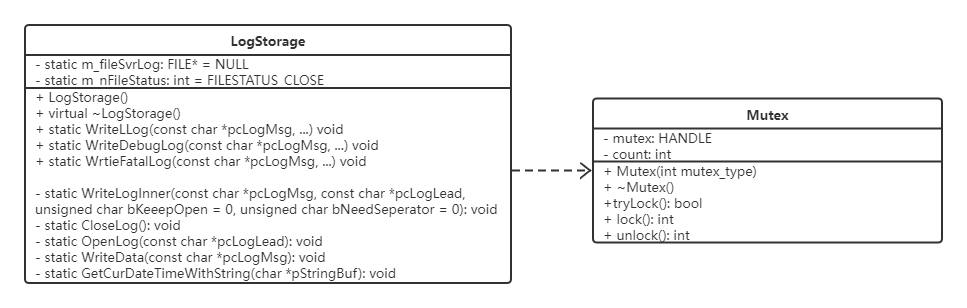
\includegraphics[width=9.67cm,height=3.08cm]{LogStorage.png}
                \caption{log system}                    
                \end{figure} 
        \subsection{DBMS design[3][4]}
            In the project, we have been schefuled to use the inner DBMS of mysql bu directly pass the operation string to the sql functions; however, in order 
            to undrstand the concpetion of BDMS, our practice is to wirte a demo which uses a folder as a database and a file as a data table.
        \subsection{Server design[5]}
            For the server end, the performing steps are: \par
            1. socket(int domain, int type,int protocol): Returns the file descriptor pointing to the newly created socket \par
            2. bind(int sockfd, const struct sockaddr *addr, socklen_t addrlen): Bind a socket to anothor socket address, namely, bind IP port(
            initialize struct sockaddr_in addr)\par
            3. listen( int sockfd, int backlog): The sockfd parameter specifies the socket to be monitored. The backlog parameter prompts the maximum length of the kernel 
            listening queue. If the length of the listening queue exceeds the backlog, the server will not accept new client connections, and the 
            client will also receive an ECONNREFUSED error message. In short, listen() specifies the maximum number of simultaneous connections \par
            4. accept(int sockfd, struct sockaddr *cliaddr, socklen_t *addrlen): The sockfd parameter is the listening socket that has executed the listen system call. The cliaddr parameter is used to 
            obtain the remote (client) socket address of the accepted connection. The length of the socket address is indicated by the addrlen 
            parameter. After the three-way handshake is completed, the server calls accept() to accept the connection. If there is no client 
            connection request when the server calls accept(), it will block and wait until a client connects. In brief, block waiting for the client to 
            initiate a connection \par
            5. read(char *operation): from client \par
            6. sql operation \par
            7. write(char *resultLog): to client \par
            8. close() \par
            For the client end, the performing steps are: \par
            1. socket() \par
            2. bind() \par
            3. connect(): connect to the server end \par
            4. write() \par
            5. read() \par
            6. close() \par
    \section{Schedule for next stage}
        First, the current system should be completed without any bugs, and our expectation is that, the user runs his programs on his personal computer, and then 
        the logs of the programs will be stored in the computer for storage. \par
        In addition to the current performance of the log storage system, it needs to be put on cloud, which is to better manage the layer structures of the 
        data center, such as seperating the computing layer and storage layer, splitting disks and adding multiple computers for storage. \par
        Finally, our test method is to use two computer for storage and two or more computers as client, and comparethe running time before and after using cloud 
        native techniques.
    \section{Reference}
        [1] https://blog.csdn.net/little_stupid_child/article/details/54708701?locationNum=5&fps=1 \par
        [2] https://blog.csdn.net/laobai1015/article/details/80004504 \par
        [3] https://blog.csdn.net/TK_wang_/article/details/106899188 \par
        [4] Database system concepts, 2020.10, China Machine Press \par
        [5] https://blog.csdn.net/qq_34201858/article/details/104139384 \par
        
    \begin{itemize}
        \item[$\bullet$] end
    \end{itemize}
\end{document}